\documentclass[12pt, a4paper]{article}

\usepackage{amsmath}
\usepackage{amsfonts}
\usepackage{amssymb}
\usepackage{graphicx}
\usepackage{float}
\usepackage{listings}
\usepackage{rotating}
\usepackage{tikz}
\usepackage{verbatim}
\pdfgentounicode=1
\pdfmapline{+cyberb@Unicode@  <cyberbit.ttf}

\begin{document}

\title{A 3D reconstruction of M.C.Escher's "House of Stairs"}
\author{P. Baillehache}
\date{\today}
\maketitle

\tableofcontents

\section{Introduction}

M.C.Escher is a Dutch graphic artist who lived from 1898 to 1972. His art is characterized by a strong bond with mathematics, and that's why I'm particularly fond of it. I've received a few reproduction as a calendar a few year ago, and among them the "House of Stairs" (ref. XL-51). This monochrom lithograph was made in 1951 and represents the interior of a building criss crossed by stairs on which salamander-like creatures crawl in chain.\\

As usual with Escher's art, the building looks at first sight odd, distorted, irrealistic. But with care it is possible to understand what's going on, and from there it became interesting to me to try to reproduce it, because as everybody knows "if you want to understand it, code it !". Then I set up the goal of creating a reproduction of this lithograph as a 3D synthesis picture.\\

If POV-Ray wasn't my natural apriori choice for making synthesis picture, mimicking the mathematical approach of the original would have been a good enough reason to use this software anyway. Thus my challenge became: reach the nearest possible reproduction of the "House of Stairs" using POV-Ray.\\

\section{First analysis of the original lithograph}

\subsection{Dimensions}

The original lithograph measures 238mm by 472mm. At 400dpi it converts to 3748px by 7433px, the size of my final image. For fast rendering during development smaller dimensions will be used: 375x743px.\\

\subsection{Colors}

The lithograph is monochrom, so a starting approximation for the texture will be white (rgb 255,255,255), a little bit rough, and the shades of gray will come from the lighting. An exception will be made for the eyes of the Curl-ups, which will be in first approximation black, highly polished and reflective.\\

\subsection{Building structure}

The House of stairs as seen by tiewer is made of 5 faces connected by stairs. Of these faces only one face (the one in front of the viewer) is entirely included in the image. Let's call this face the front wall.\\

The face on the left side of the image will be called the left wall, the one on the right side of the image will be called the right wall, the one on the center bottom will be called the bottom wall, and the one on the center top of the image will be called the top wall.\\

\begin{center}
\begin{figure}[H]
\centering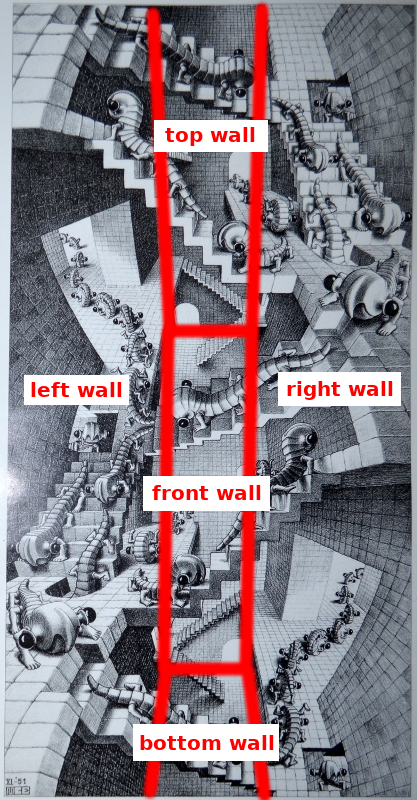
\includegraphics[width=6cm]{./walls.png}\\
\end{figure}
\end{center}

One can notice the symmetry in the visible portion of the walls. The top wall is the horizontal mirrored image of the bottom of the front wall, and the bottom wall is the horizontal mirrored image of the top of the front wall. This symmetry applies also to the Curl-ups, with the exception of the top-right and bottom-right corners of the image, where two other Curl-ups should be present to preserve the symmetry.\\

\begin{center}
\begin{figure}[H]
\centering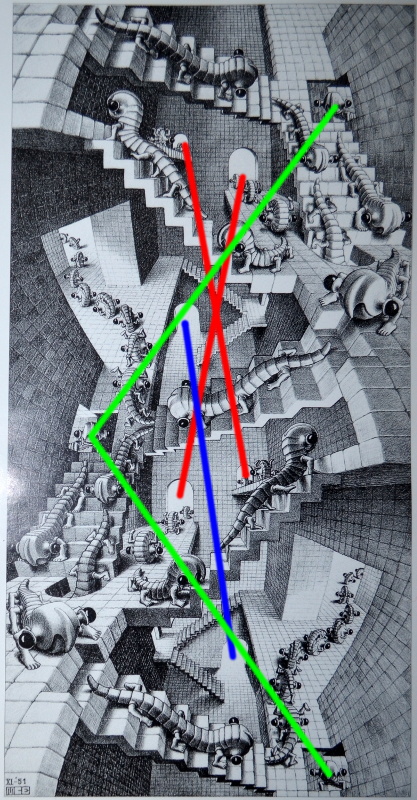
\includegraphics[width=6cm]{./mirror.png}\\
\end{figure}
\end{center}

\begin{center}
\begin{figure}[H]
\centering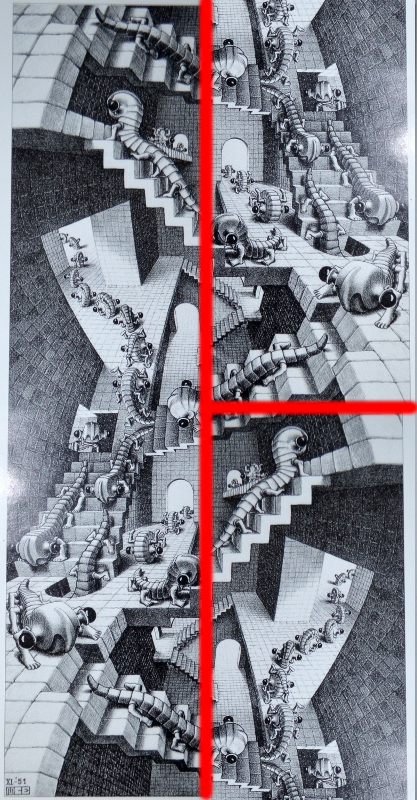
\includegraphics[width=6cm]{./mirror2.png}\\
\end{figure}
\end{center}

From the two observations above I'll make the following hypothesis:\\

\emph{Hypothesis 1: the right side of the image is the horizontal mirrored image of the left side of the image, shifted along the top-bottom axis.}\\

Next we can also notice that the top of the image repeats the bottom of the image.\\

\begin{center}
\begin{figure}[H]
\centering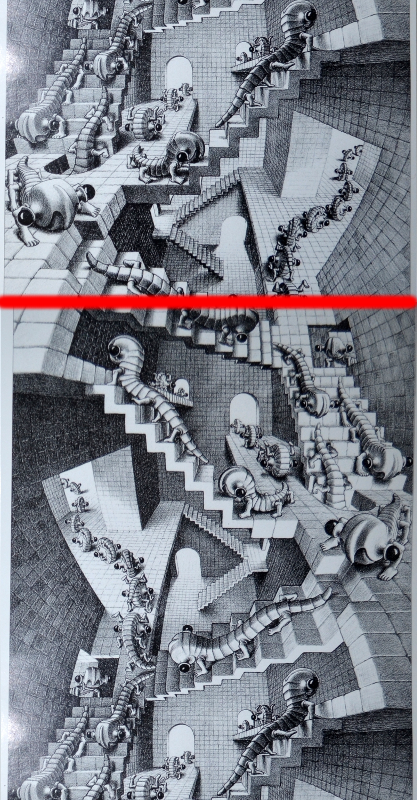
\includegraphics[width=6cm]{./mirror3.png}\\
\end{figure}
\end{center}

Which leads to another hypothesis:\\

\emph{Hypothesis 2: the image repeats infinitely along the top-bottom axis.}\\

On the base of the following observation, I'll make another hypothesis: the walls which looks concave in the image are actually flat rectangles at right angle from one another, and looks concave due to the optical properties of the viewer.\\

\emph{Hypothesis 3: walls are flat rectangles at right angle from one another.}\\

If the previous hypothesis are true, the building is actually a paralellepiped whose left half section is the symmetry of the right half section rotated by 90 degrees relatively to the left-right axis in the image passing through its center.\\

\subsection{Building dimensions}

The building's wall is almost (exception for the doors and stairs) entirely made of supposedly cubic blocks. Without any other indication for sizes, I'll take it as my reference. So the unit of measure will be one block (1bl) and I make the following hypothesis:\\

\emph{Hypothesis 3: the blocks the walls are made of are cubes.}\\

The size of the front wall along the left-right axis can be directly measured: it's 25bl.\\

However its size along the up-down axis can't directly be measured as the stairs partially hide the front wall. However, it is possible to measure it by using the previous hypothesis: invisible portions of the front wall can be deducted by its equivalent in repeated top/bottom walls and mirrored side of the image. It's 102bl.\\

\begin{center}
\begin{figure}[H]
\centering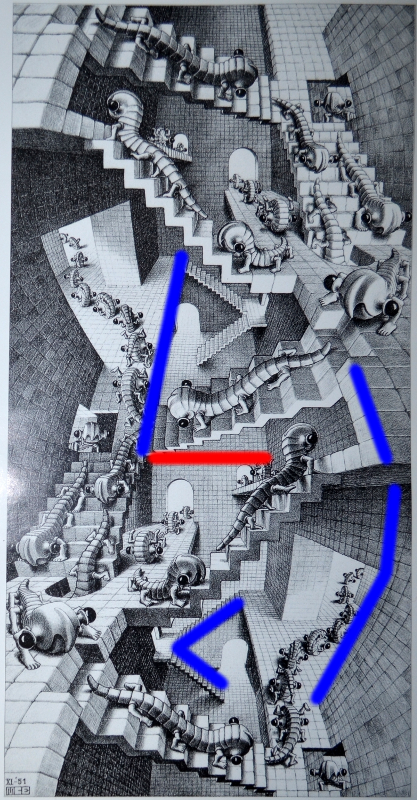
\includegraphics[height=10cm]{./dimension.png}\\
\end{figure}
\end{center}

\subsection{View point}

By tracing the diagonals of the lithograph and those of the front wall we see that the viewer stands aligned with the center of the front wall along the left-right axis, but is shifted along the top-down axis toward the bottom of the image.\\

\begin{center}
\begin{figure}[H]
\centering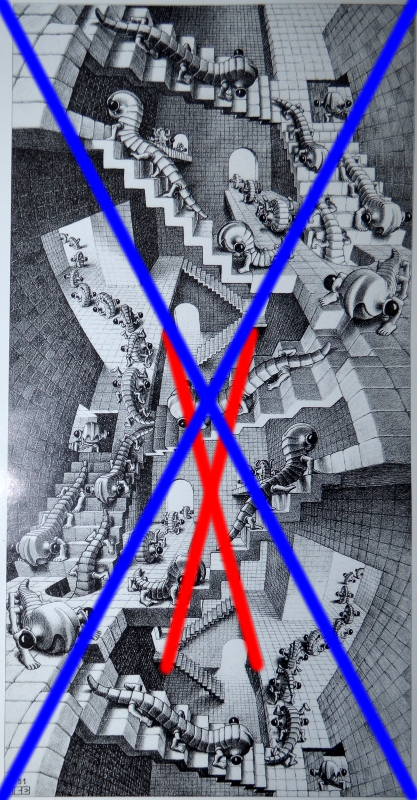
\includegraphics[height=10cm]{./viewpoint.png}\\
\end{figure}
\end{center}

Without any other information I'll make the following hypothesis:\\

\emph{Hypothesis 4: the view point is located at the center of the House of stairs, looking toward the front wall, at its center along left-right axis, and one quarter of its length from its top in the image.}\\

Following the previous hypothesis I can infer some properties of the optic of the viewer: an ultra wide lens spanning 180 degrees along left-right and top-bottom axis.\\

\section{Prototype in POV-Ray}

I've first make a prototype model of the walls without doors, stairways, platforms and Curl-ups to verify the hypothesis about the optic and dimensions. It comes as follow:\\

\begin{scriptsize}
\begin{ttfamily}
\lstinputlisting[breaklines]{./XL-51_1.pov}
\end{ttfamily}
\end{scriptsize}

\begin{center}
\begin{figure}[H]
\centering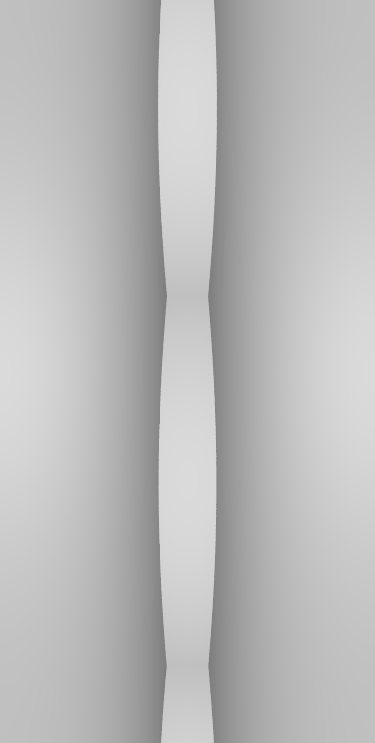
\includegraphics[height=10cm]{./XL-51_1.png}\\
\end{figure}
\end{center}

A superposition with the lithography shows that the model is globally correct but the front, top, bottom walls are half too narrow. The top and bottom of the front wall also don't match the original ones.\\

\begin{center}
\begin{figure}[H]
\centering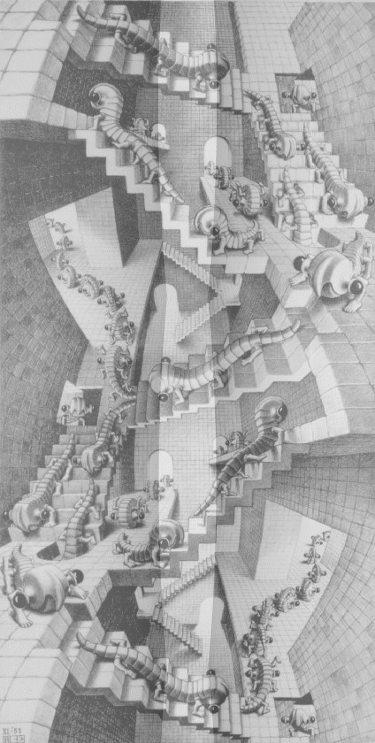
\includegraphics[height=10cm]{./checkDimensionViewPoint_1.png}\\
\end{figure}
\end{center}

Looking at the block of the platform on the center right of the lithography I add another hypothesis:\\

\emph{Hypothesis 4: one block unit along the left-rght axis is twice as long as one block unit along the top-bottom axis.}\\

Then I tune empirically the angle of the ultra wide lens (200 degrees), and the position of the view point (0.2375 * lengthRoom from the top of the fron wall). Which brings to a satisfying approximation of the room.\\

\begin{scriptsize}
\begin{ttfamily}
\lstinputlisting[breaklines]{./XL-51_2.pov}
\end{ttfamily}
\end{scriptsize}

\begin{center}
\begin{figure}[H]
\centering
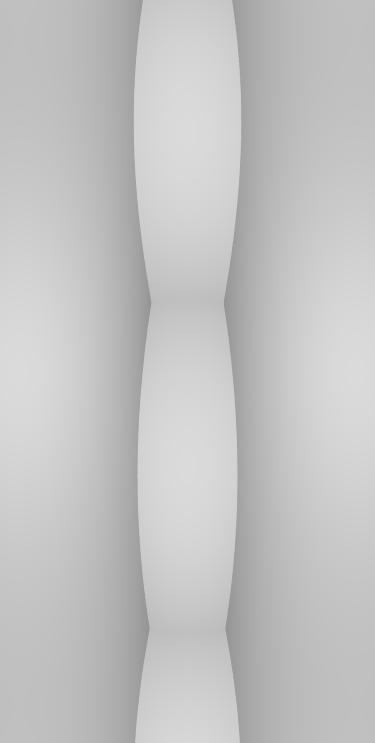
\includegraphics[height=10cm]{./XL-51_2.png}
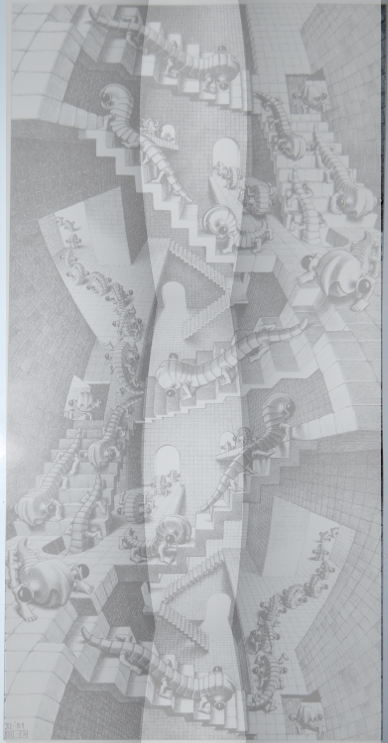
\includegraphics[height=10cm]{./checkDimensionViewPoint_2.png}\\
\end{figure}
\end{center}

To give more credit to my hypothesis, I add the right platform and check it matches the lithography. The dimension of the right platform are 50bl long, 10bl large and 1bl thick. It's also 52bl away from the bottom of the front wall. I also replace the white texture with a checker texture to visualize more easily the deformation of the wall through the wide angle lens.\\

\begin{scriptsize}
\begin{ttfamily}
\lstinputlisting[breaklines]{./XL-51_3.pov}
\end{ttfamily}
\end{scriptsize}

\begin{center}
\begin{figure}[H]
\centering
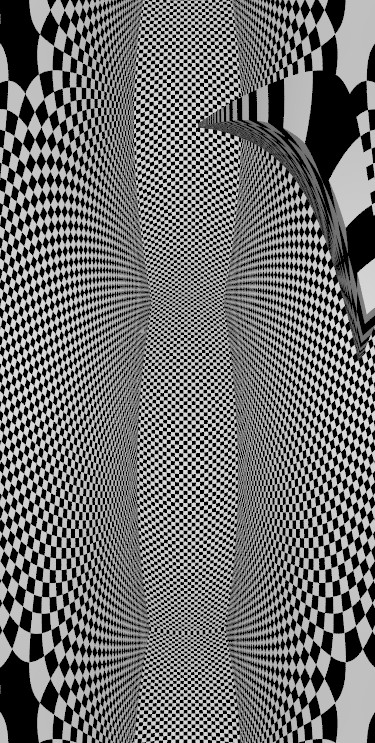
\includegraphics[height=10cm]{./XL-51_3.png}\\
\end{figure}
\end{center}

Now I see that the wide angle lens hypothesis is incorrect: in the lithography the horizontal lines are straight but ine the rendered image they are curved. Also, from the position of the platform I see that the camera position is probably not right at the center of the House.\\

I first try with another type of projection for the camera: the cylinder projection.\\

\begin{scriptsize}
\begin{ttfamily}
\lstinputlisting[breaklines]{./XL-51_4.pov}
\end{ttfamily}
\end{scriptsize}

\begin{center}
\begin{figure}[H]
\centering
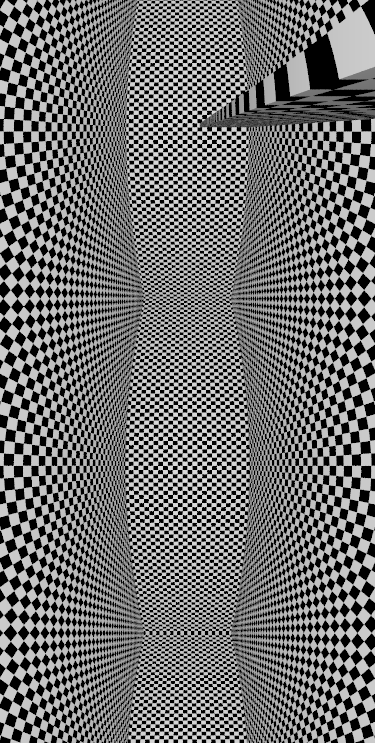
\includegraphics[height=10cm]{./XL-51_4.png}\\
\end{figure}
\end{center}

The projection looks much better. Now I try to improve the camera position.\\

\begin{scriptsize}
\begin{ttfamily}
\lstinputlisting[breaklines]{./XL-51_5.pov}
\end{ttfamily}
\end{scriptsize}

\begin{center}
\begin{figure}[H]
\centering
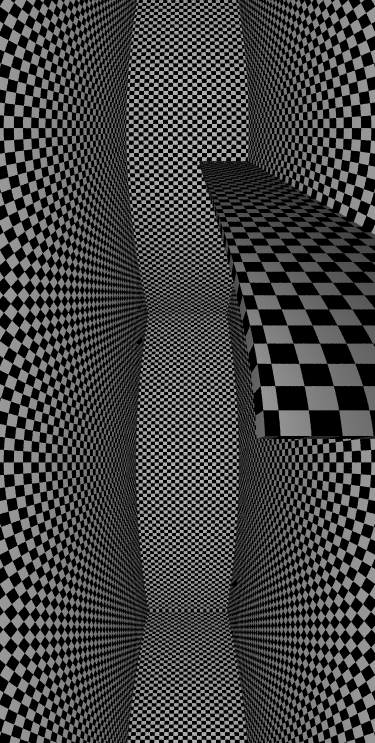
\includegraphics[height=10cm]{./XL-51_5.png}
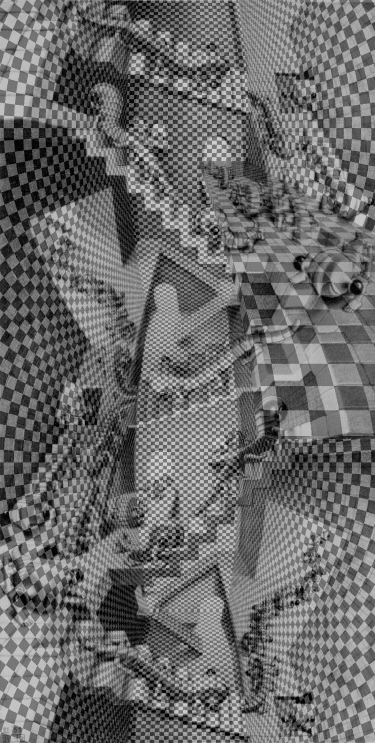
\includegraphics[height=10cm]{./checkDimensionViewPoint_3.png}\\
\end{figure}
\end{center}

Now the rendered image matches the lithography enough for now and I want to confirm the symmetry hypothesis. Then I change the script to create the House by repeating, rotating and mirroring the platform and one fourth of the walls.\\

\begin{scriptsize}
\begin{ttfamily}
\lstinputlisting[breaklines]{./XL-51_6.pov}
\end{ttfamily}
\end{scriptsize}

\begin{center}
\begin{figure}[H]
\centering
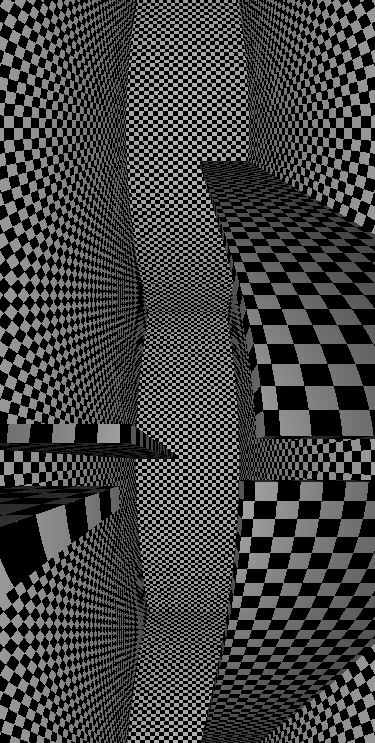
\includegraphics[height=10cm]{./XL-51_6.png}\\
\end{figure}
\end{center}

The repeated platforms doesn't match the ones in the lithography. My guess is that I've mistaken its dimensions (and consequently the position of the camera should also be wrong). I now try to correct this.\\

\begin{scriptsize}
\begin{ttfamily}
\lstinputlisting[breaklines]{./XL-51_7.pov}
\end{ttfamily}
\end{scriptsize}

\begin{center}
\begin{figure}[H]
\centering
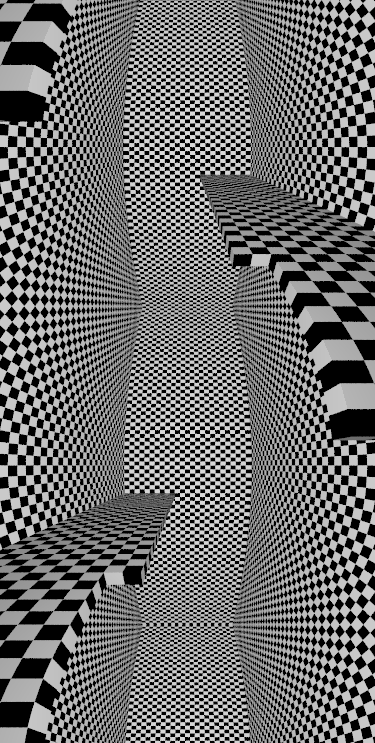
\includegraphics[height=10cm]{./XL-51_7.png}
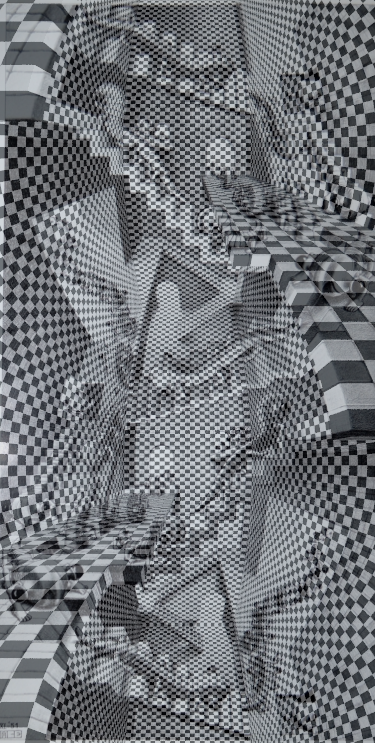
\includegraphics[height=10cm]{./checkDimensionViewPoint_4.png}\\
\end{figure}
\end{center}

Getting closer and closer to the right dimensions for the House and parameters for the camera. Now I add the two other platforms, again using symetry. Their dimensions can be easily deducted from the first platform.\\

\begin{scriptsize}
\begin{ttfamily}
\lstinputlisting[breaklines]{./XL-51_8.pov}
\end{ttfamily}
\end{scriptsize}

\begin{center}
\begin{figure}[H]
\centering
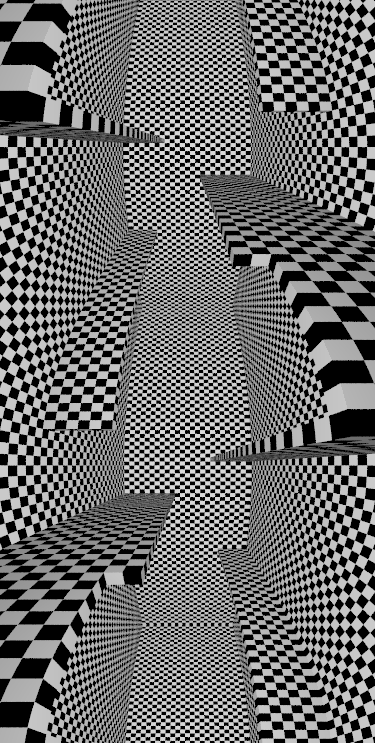
\includegraphics[height=10cm]{./XL-51_8.png}\\
\end{figure}
\end{center}

Next, I confirm and eventually correct the dimensions of the platforms by adding some simple models for the stairs connecting the platforms.\\

\begin{scriptsize}
\begin{ttfamily}
\lstinputlisting[breaklines]{./XL-51_9.pov}
\end{ttfamily}
\end{scriptsize}

\begin{center}
\begin{figure}[H]
\centering
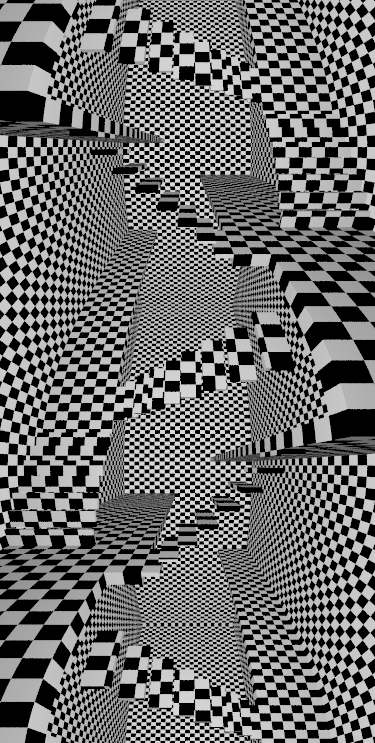
\includegraphics[height=10cm]{./XL-51_9.png}\\
\end{figure}
\end{center}

The stairs and platform fit very well altogether, but there is some deviation between the image and the lithography. I believe it will be solved by tuning again the camera parameters.\\

I think it's enough for the prototype. The remaining stairs, doors and external walls should not cause problems given what matches so well in the prototype. So I move on to the real model.\\

\section{Final model in POV-Ray}

\subsection{Block model}

As the basic element of the house is the block I start by creating its model and a macro to generate walls made of these blocks.\\

\begin{scriptsize}
\begin{ttfamily}
\lstinputlisting[breaklines]{./block_1.pov}
\end{ttfamily}
\end{scriptsize}

\begin{center}
\begin{figure}[H]
\centering
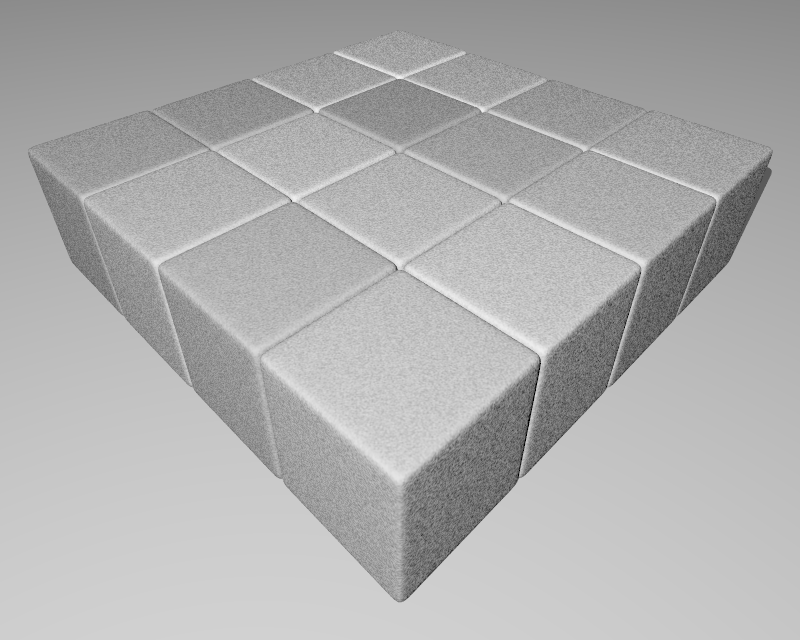
\includegraphics[width=6cm]{./block_1.png}\\
\end{figure}
\end{center}

\subsection{Cleaning the prototype script}

In preparation for the refactoring of the prototype of the House of Stairs I clean its script.\\

blocks.inc:\\
\begin{scriptsize}
\begin{ttfamily}
\lstinputlisting[breaklines]{./blocks_1.inc}
\end{ttfamily}
\end{scriptsize}

XL-51.pov:\\
\begin{scriptsize}
\begin{ttfamily}
\lstinputlisting[breaklines]{./clean_prototype.pov}
\end{ttfamily}
\end{scriptsize}

\begin{center}
\begin{figure}[H]
\centering
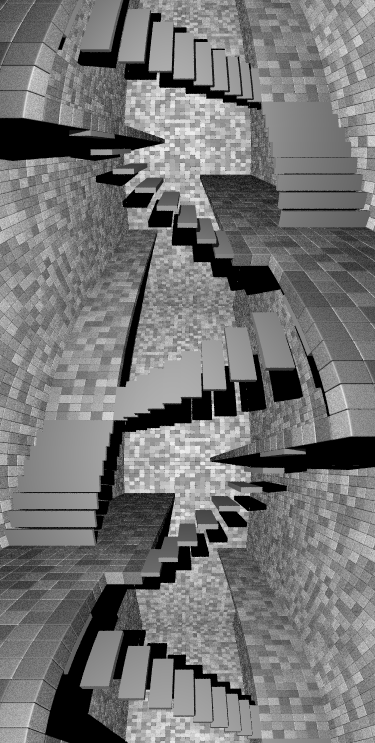
\includegraphics[width=6cm]{./clean_prototype.png}\\
\end{figure}
\end{center}

\subsection{Stair model}

I finish the model for the stairs.\\

blocks.inc:\\
\begin{scriptsize}
\begin{ttfamily}
\lstinputlisting[breaklines]{./blocks_2.inc}
\end{ttfamily}
\end{scriptsize}

XL-51.pov:\\
\begin{scriptsize}
\begin{ttfamily}
\lstinputlisting[breaklines]{./XL-51_10.pov}
\end{ttfamily}
\end{scriptsize}

\begin{center}
\begin{figure}[H]
\centering
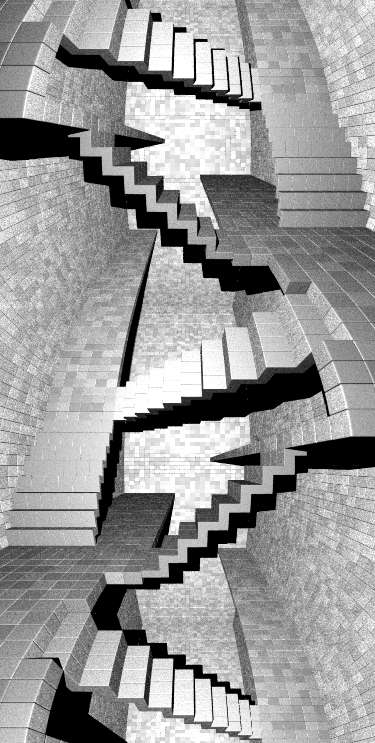
\includegraphics[width=6cm]{./XL-51_10.png}\\
\end{figure}
\end{center}

It looks nice but looking closely at the stairs make me realize it doesn't match the lithography. There is a problem in dimensions or position of the platforms. I try to fix that, refactor completely the dimensions of my model, and doing so start to find inconsistencies in the drawing.\\

First, the horizontal dimension of the front wall doens't match in its upper part and center part (24 blocks against 25 blocks).\\

\begin{center}
\begin{figure}[H]
\centering
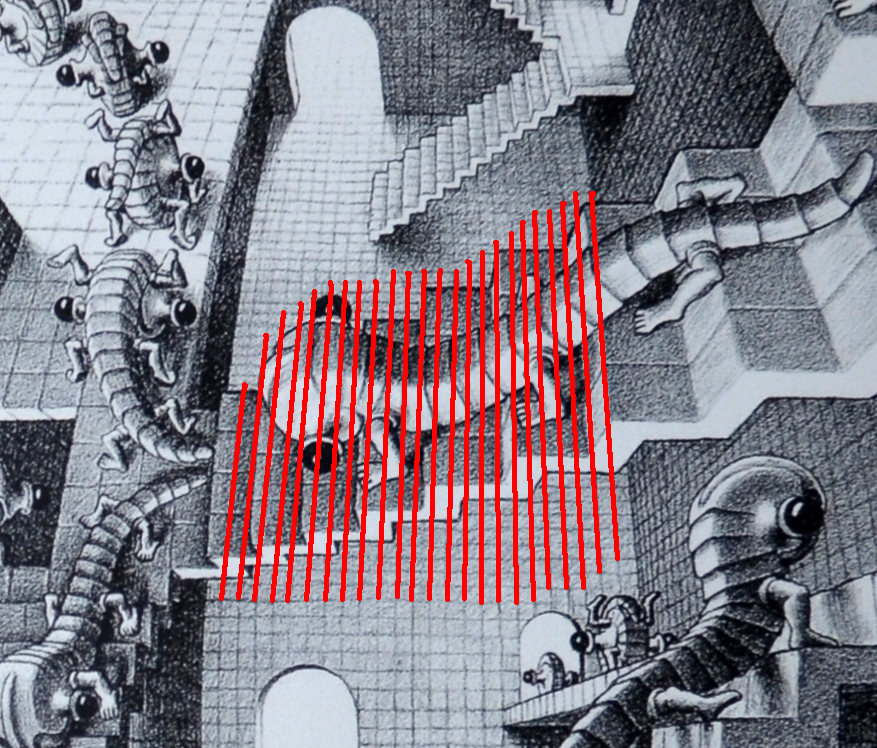
\includegraphics[width=6cm]{./inconsistency_1.png}\\
\end{figure}
\end{center}

Second, the red and blue lines below should have same dimension along the depth axis but they haven't (10 blocks against 9 blocks).\\

\begin{center}
\begin{figure}[H]
\centering
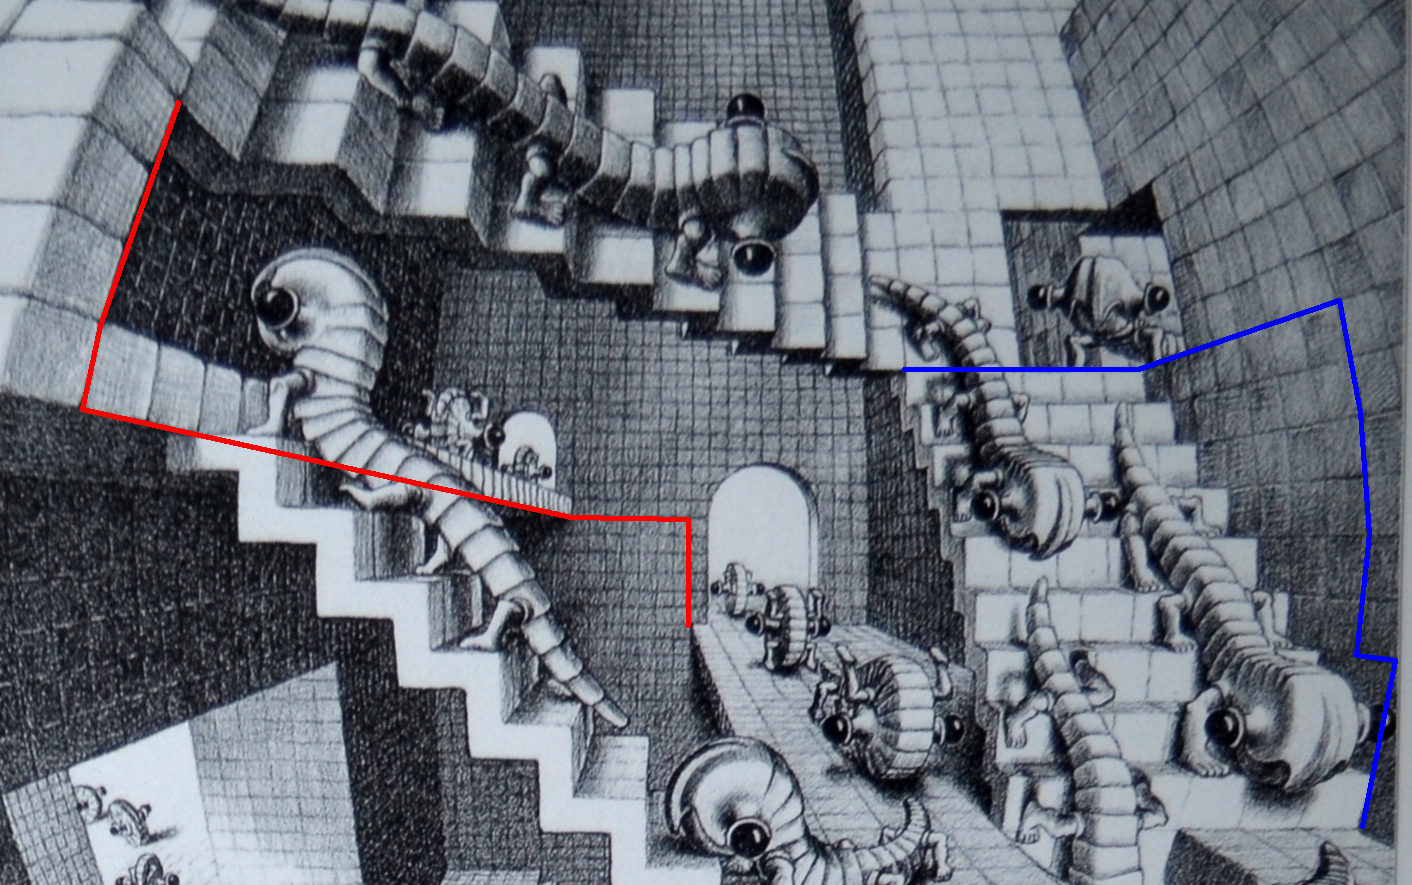
\includegraphics[width=6cm]{./inconsistency_2.png}\\
\end{figure}
\end{center}

I'm really embarrassed. If the drawing is mathematically incorrect I have no way to reproduced it exactly in Pov-Ray... I have no choice but to find a compromise. I rework once again the dimensions of the model.\\

\end{document}


